\subsection{Exemples de calcul de $E_p$}

$\vec{F} =-kx\vec{i}$ Force de rappel \ul{elastique}

$\vec{F}$ est elle conservative ? .
\[\begin{array}{rcl}
F &=& -kx \\
&=& -d\frac{E_p}{dx} \\
dE_p &=& -Fd_x = -(-kx=dx \\
E_p(x) &=& \int kxdx \\
&=& \frac{1}{2}dx^2 + c\end{array}\]

Si on prend l'origine des $E_p$ en $x=0$, alors $E_p(x) = \frac{1}{2}kx^2$ \textbf{Energie potentiel elastique}

\paragraph{force de pensanteur}

\begin{wrapfigure}[6]{r}{0pt}
	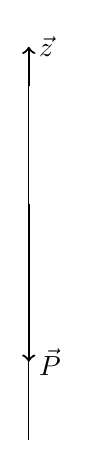
\begin{tikzpicture}
		\draw[] (0, 0) -- (0, 5);
		\draw[->, thick] (0, 4.5) -- (0, 5) node [right] {$\vec{z}$};
		\draw[->, thick] (0, 3) -- (0, 1) node [right] {$\vec{P}$};
	\end{tikzpicture}
\end{wrapfigure}

\[\begin{array}{rcl}
\vec{P} &=& -mg\vec{k} \\
\text{Si F est conservative } F &=& -\frac{dE_p(z)}{dz} \\
dE_p(z) &=& -Fdz \\
\text{ et } F &=& P = -mg \\
dE_p(z) &=& -(-mg)dz \\
E_p(z) &=& mgz + C \\
\text{Si } E_p(0) &=& 0 \Rightarrow E_p(z) = mgz\end{array}\]

\subsection{force de frottement visqueux}

\begin{wrapfigure}[5]{r}{0pt}
\begin{tikzpicture}
	\draw[fill=gray, opacity=0.5] (0, 0) rectangle (4, 2);
	\draw[fill=black] (2, 1) circle (0.05);
	\draw[thick] (2, 1) -- (1, 1) node [above] {$\vec{f}$};
	\draw[thick] (2, 1) -- (3, 1) node [above] {$\vec{v}$};
\end{tikzpicture}

\end{wrapfigure}

\[\begin{array}{rclr}
	\vec{f} &=& -\lambda \vec{v} \\
	f &=& -\lambda \dot{x} & ? \exists E_p(x) \text{ tel que } (-\lambda \cdot{x}) = -\frac{E_p}{dx}
\end{array}\]

Impossible car dépend de la vitesse, donc du temps et du chemin parcourue.

\section{Energie Mecanique}

Il y a deux type d'énergie : l'énergie cinétique $E_c = \frac{1}{2}mv^2$, l'énergie potentielle $E_p(x)$

L'énergie Mécanique est défini comme étant : 
\begin{center}
	\fbox{$E_m=E_p+E_c$}
\end{center}

\subsection{Théorème d'énergie mécanique}
Soit $m$ soumise à des $\vec{F}$ conservative $\vec{F_c}$ et des $\vec{f}$ non conservative $\vec{F_{nc}}$

\[\delta E_c = \sum_i W(\vec{F_i}) = \sum_{i_1} W(\vec{F_{i_1c}}) + \sum_{i_2} W(\vec{F_{i_2 nc}})\]

\[\begin{array}{rcl}
\text{ or } \sum_{i_1}W_{A \to B}(\vec{F_{i_1c}}) &=& E_p(A)-E_p(B) \\
\delta_{A \to B} E_c &=& E_c(B) - E_c(A) = E_p(A)-E_p(B) + \sum_{i_2} W(\vec{F_{i_2 nc}}) \\
{[E_c(B) + E_p(B)]} - {[E_c(A) + E_p(A)]} &=& \sum_{i_2} (\vec{F_{i_2nc}})\end{array}\]

\paragraph{Enonce} La variation de l'énergie mécanique est égale à la somme des travaux des forces non conservative.

\begin{center}
	\fbox{$E_m(B) - E_m(A) = \sum_{i_2}W(\vec{F_{i_2nc}})$}
\end{center}

\paragraph{Conséquence} En absence de forces non conservative, l'énergie mécanique est constante du mouvement.

\subsection{Forme locale du theoreme d'énergie mécanique}

\[\begin{array}{rcl}
	E_m &=& E_c + E_p \\
	dE_m &=& dE_c + dE_p \\
	\frac{dE_m}{dt} &=& \frac{dE_c}{dt} + \frac{dE_p}{dt} \\
	\frac{dE_m}{dt} &=& \frac{d(\frac{1}{2}mv^2)}{dt} \\
&=& \frac{1}{2}m\frac{d}{dt}(v^2) \\
&=& \frac{1}{2}m(2v\cdot \dot{v}) \\
\frac{dE_m}{dt} &=& (m\dot{v})v = f \cdot v \end{array}\]

en \ul{3D} \fbox{$\frac{dE_m}{dt} = \vec{f}\cdot \vec{v}$} avec $\vec{f}$ la résultante des forces.

\subsection{Applications $E_m$ en absence de frottement}

\begin{wrapfigure}{r}{0pt}
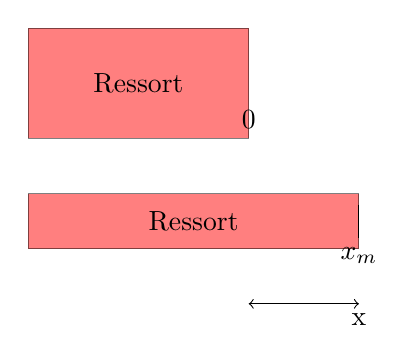
\begin{tikzpicture}[scale=0.7]
	\draw[fill=red, opacity=0.5] (0, 2) rectangle (4, 0);
	\node at (2, 1) {Ressort};
	\draw[fill=red, opacity=0.5] (0, -1) rectangle (6, -2);
	\draw[<->] (4, -3) -- (6, -3) node [below] {x};
	\node at (3, -1.5) {Ressort};
	\draw[] (6, -1.2) -- (6, -1.8) node [below] {$x_m$};
	\node [above] at (4, 0) {0};
\end{tikzpicture}
\end{wrapfigure}
$\begin{array}{rcl}
	\text{Cas du ressort : } E_m &=& E_p + E_c \\
&=& \frac{1}{2}kx^2 + \frac{1}{2}m\dot{x}^2\end{array}$

Quelle est sa vitesse maximal $v_{max}$ et où ?
Position initiale : $x_m$, $v_i = 0$

\[E_{mi} = 0 + \frac{1}{2}k(x_m^2)\]

Quand v est maximal :

\[\begin{array}{rcl}
	E_{m_f} &=& \frac{1}{2}mv^2_{max} + \frac{1}{2}(kx_0^2) \\
	&=& \frac{1}{2}kx_m^2 \\
\frac{1}{2}mv_m^2 + \frac{1}{2}(kx_0^2) &=& C \end{array}\]

Donc $v_m$ est maximal quand $x_0^2$ est minimal : $x_0 = 0$.
\[\begin{array}{rcl}
	\frac{1}{2} mv_m^2 &=& \frac{1}{2}kx_m^2 \\
v_m &=& \sqrt{\frac{k}{m}}x_m\end{array}\]

\paragraph{} Calculer l'énergie potentielle d'un satellite dans le champ de gravitation de la terre en absence de frottement avec l'atmosphère, $E_p(\infty) = 0$

\paragraph{} Celle d'une comète et d'une planète. $v_0 = 0$, $E_p(\infty) = 0$
